\documentclass[a4paper]{paper}

\usepackage{fullpage}
\usepackage[utf8]{inputenc}
\usepackage[T1]{fontenc}
\usepackage{amsthm}

\usepackage{color}
\newcommand{\xcol}{blue}
\newcommand{\ycol}{red}

\usepackage{tikz}

\newcommand{\nomFormat}{Fodaly}
\newtheorem{definition}{Definition}


\title{\nomFormat{}~: description textuelle de labyrinthes}
%\author{L. Jezequel}
%\date{Le 23 mai 2016}

\author{\textrm{Projet} \textsf{Tremplin en DUT informatique},
\textrm{IUT de Nantes}}



\begin{document}

\maketitle

\section{Grilles, murs, arènes, labyrinthes}

On considère des \emph{grilles} constituées de cases, auxquelles on associe des coordonnées : une abscisse ($x$) et une ordonnée ($y$).
La figure~\ref{fig:grille} (gauche) donne un exemple d'une telle grille.
La case repérée par un X a pour abscisse $2$ et pour ordonnée $1$, on dira donc que c'est la case de coordonnées $(2, 1)$. Notons qu'on commence la numérotation par 0.

On peut placer des \emph{murs} sur les cases d'une telle grille.
Sur la figure~\ref{fig:grille} (droite), les murs sont représentés par des cases pleines.

\begin{figure}[htbp]
  \centering
  \scalebox{0.8}{%
  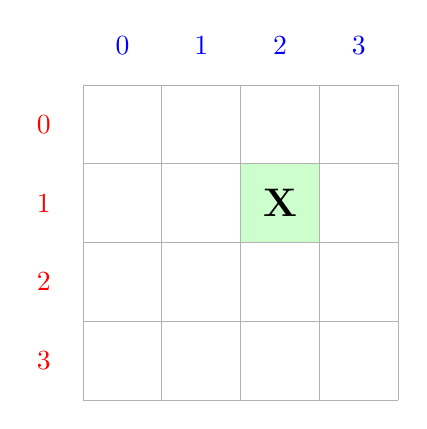
\begin{tikzpicture}

    \node[\xcol] (x1) at (0.5, 0.5) {0};
    \node[\xcol] (x2) at (1.5, 0.5) {1};
    \node[\xcol] (x3) at (2.5, 0.5) {2};
    \node[\xcol] (x3) at (3.5, 0.5) {3};

    \node[\ycol] (y1) at (-0.5, -0.5) {0};
    \node[\ycol] (y2) at (-0.5, -1.5) {1};
    \node[\ycol] (y3) at (-0.5, -2.5) {2};
    \node[\ycol] (y3) at (-0.5, -3.5) {3};


    % exemple de case
    \draw[fill=green!20, draw=none] (2, -1) rectangle (3, -2);
    \node (x) at (2.5, -1.5) {{\Large\bf X}};

    \draw[draw=black!30] (0, 0) -- (4, 0);
    \draw[draw=black!30] (0, -1) -- (4, -1);
    \draw[draw=black!30] (0, -2) -- (4, -2);
    \draw[draw=black!30] (0, -3) -- (4, -3);
    \draw[draw=black!30] (0, -4) -- (4, -4);
    \draw[draw=black!30] (0, 0) -- (0, -4);
    \draw[draw=black!30] (1, 0) -- (1, -4);
    \draw[draw=black!30] (2, 0) -- (2, -4);
    \draw[draw=black!30] (3, 0) -- (3, -4);
    \draw[draw=black!30] (4, 0) -- (4, -4);

  \end{tikzpicture}}
  \hspace{3cm}
  \scalebox{0.8}{%
  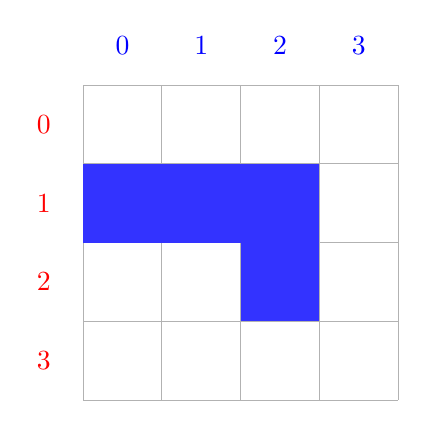
\begin{tikzpicture}

    \node[\xcol] (x1) at (0.5, 0.5) {0};
    \node[\xcol] (x2) at (1.5, 0.5) {1};
    \node[\xcol] (x3) at (2.5, 0.5) {2};
    \node[\xcol] (x3) at (3.5, 0.5) {3};

    \node[\ycol] (y1) at (-0.5, -0.5) {0};
    \node[\ycol] (y2) at (-0.5, -1.5) {1};
    \node[\ycol] (y3) at (-0.5, -2.5) {2};
    \node[\ycol] (y3) at (-0.5, -3.5) {3};

    \draw[draw=black!30] (0, 0) -- (4, 0);
    \draw[draw=black!30] (0, -1) -- (4, -1);
    \draw[draw=black!30] (0, -2) -- (4, -2);
    \draw[draw=black!30] (0, -3) -- (4, -3);
    \draw[draw=black!30] (0, -4) -- (4, -4);
    \draw[draw=black!30] (0, 0) -- (0, -4);
    \draw[draw=black!30] (1, 0) -- (1, -4);
    \draw[draw=black!30] (2, 0) -- (2, -4);
    \draw[draw=black!30] (3, 0) -- (3, -4);
    \draw[draw=black!30] (4, 0) -- (4, -4);

    % exemple de murs
    \draw[fill=blue!80, draw=none] (0, -1) rectangle (1, -2);
    \draw[fill=blue!80, draw=none] (1, -1) rectangle (2, -2);
    \draw[fill=blue!80, draw=none] (2, -1) rectangle (3, -2);
    \draw[fill=blue!80, draw=none] (2, -2) rectangle (3, -3);

  \end{tikzpicture}}
\caption{Une grille, des murs sur une grille, une arène, un labyrinthe}\label{fig:grille}
\end{figure}


\begin{definition}{(arène)}
On appelle une \emph{arène} une grille équipée de murs.
\end{definition}

Pour constituer un labyrinthe on rajoute des murs autour de la grille (à l'extérieur, comme sur la figure~\ref{fig:grille2} (gauche).

On ajout aussi un point de départ et un point d'arrivée sur des cases de la grille.

\begin{definition}{(\emph{labyrinthe})}
Un labyrinthe est une arène, avec  un point de départ (D) et un point d'arrivée (A) et qui a été entièrement entourée de murs.%, et telle qu'il est possible en partant du point de départ, d'atteindre le point d'arrivée en se déplaçant entre cases adjacentes sans jamais couper un mur.
%En ajoutant un point de départ et un point d'arrivée à une arène on obtient un \emph{labyrinthe}, à condition qu'il soit possible d'atteindre l'arrivée depuis le départ en se déplacent entre cases adjacentes sans jamais couper un mur.
\end{definition}

Sur la figure~\ref{fig:grille2} (droite) un labyrinthe est représenté.
Le départ est noté D (coordonnées (0,0)) et l'arrivée A (coordonnées (3,3)).



\begin{figure}[htbp]
  \centering
  \scalebox{0.8}{%
  
\begin{tikzpicture}

    \node[\xcol] (x1) at (0.5, 0.5) {0};
    \node[\xcol] (x2) at (1.5, 0.5) {1};
    \node[\xcol] (x3) at (2.5, 0.5) {2};
    \node[\xcol] (x3) at (3.5, 0.5) {3};

    \node[\ycol] (y1) at (-0.5, -0.5) {0};
    \node[\ycol] (y2) at (-0.5, -1.5) {1};
    \node[\ycol] (y3) at (-0.5, -2.5) {2};
    \node[\ycol] (y3) at (-0.5, -3.5) {3};

    \draw[draw=black!30] (0, 0) -- (4, 0);
    \draw[draw=black!30] (0, -1) -- (4, -1);
    \draw[draw=black!30] (0, -2) -- (4, -2);
    \draw[draw=black!30] (0, -3) -- (4, -3);
    \draw[draw=black!30] (0, -4) -- (4, -4);
    \draw[draw=black!30] (0, 0) -- (0, -4);
    \draw[draw=black!30] (1, 0) -- (1, -4);
    \draw[draw=black!30] (2, 0) -- (2, -4);
    \draw[draw=black!30] (3, 0) -- (3, -4);
    \draw[draw=black!30] (4, 0) -- (4, -4);

    % exemple de murs
    \draw[fill=blue!80, draw=none] (0, -1) rectangle (1, -2);
    \draw[fill=blue!80, draw=none] (1, -1) rectangle (2, -2);
    \draw[fill=blue!80, draw=none] (2, -1) rectangle (3, -2);
    \draw[fill=blue!80, draw=none] (2, -2) rectangle (3, -3);

    % contours
    \draw[fill=blue!80, draw=none] (-1, 1) rectangle (5, 0);
    \draw[fill=blue!80, draw=none] (4, 1) rectangle (5, -5);
    \draw[fill=blue!80, draw=none] (-1, -4) rectangle (5, -5);
    \draw[fill=blue!80, draw=none] (-1, 1) rectangle (0, -5);

  \end{tikzpicture}}
  \hspace{3cm}
  \scalebox{0.8}{%
  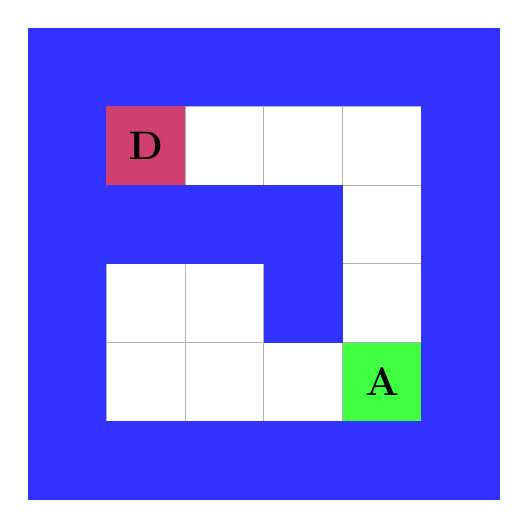
\begin{tikzpicture}


        \node[\xcol] (x1) at (0.5, 0.5) {0};
        \node[\xcol] (x2) at (1.5, 0.5) {1};
        \node[\xcol] (x3) at (2.5, 0.5) {2};
        \node[\xcol] (x3) at (3.5, 0.5) {3};

        \node[\ycol] (y1) at (-0.5, -0.5) {0};
        \node[\ycol] (y2) at (-0.5, -1.5) {1};
        \node[\ycol] (y3) at (-0.5, -2.5) {2};
        \node[\ycol] (y3) at (-0.5, -3.5) {3};

        \draw[draw=black!30] (0, 0) -- (4, 0);
        \draw[draw=black!30] (0, -1) -- (4, -1);
        \draw[draw=black!30] (0, -2) -- (4, -2);
        \draw[draw=black!30] (0, -3) -- (4, -3);
        \draw[draw=black!30] (0, -4) -- (4, -4);
        \draw[draw=black!30] (0, 0) -- (0, -4);
        \draw[draw=black!30] (1, 0) -- (1, -4);
        \draw[draw=black!30] (2, 0) -- (2, -4);
        \draw[draw=black!30] (3, 0) -- (3, -4);
        \draw[draw=black!30] (4, 0) -- (4, -4);

        % exemple de murs
        \draw[fill=blue!80, draw=none] (0, -1) rectangle (1, -2);
        \draw[fill=blue!80, draw=none] (1, -1) rectangle (2, -2);
        \draw[fill=blue!80, draw=none] (2, -1) rectangle (3, -2);
        \draw[fill=blue!80, draw=none] (2, -2) rectangle (3, -3);

        % contours
        \draw[fill=blue!80, draw=none] (-1, 1) rectangle (5, 0);
        \draw[fill=blue!80, draw=none] (4, 1) rectangle (5, -5);
        \draw[fill=blue!80, draw=none] (-1, -4) rectangle (5, -5);
        \draw[fill=blue!80, draw=none] (-1, 1) rectangle (0, -5);

        % départ
        \draw[fill=purple!75, draw=none] (0, 0) rectangle (1, -1);
        \node (d) at (0.5, -0.5) {{\Large\bf D}};

        % arrivée
        \draw[fill=green!75, draw=none] (3, -3) rectangle (4, -4);
        \node (a) at (3.5, -3.5) {{\Large\bf A}};

  \end{tikzpicture}}
  \caption{Une grille, des murs sur une grille, une arène, un labyrinthe}\label{fig:grille2}
\end{figure}

Le reste de ce document présente le format de fichier \nomFormat{}, permettant de décrire des arènes.

\section{Le format \nomFormat{}}

\subsection{Principe de base}
\label{section:base}

On ne va décrire que les arènes dans le format textuel \nomFormat{}.
C'est-à-dire qu'on ne placera pas le point de départ et d'arrivée, et qu'on ne décrira pas les murs qui doivent entourer l'arène pour former un labyrinthe.

Pour décrire une arène par un fichier texte on procédera ligne par ligne (et de haut en bas)~: chaque ligne de l'arène sera représentée par une ligne de texte.
De même, pour chaque ligne on procédera case par case (et de gauche à droite)~: chaque case sera représentée par un caractère.
Comme nos cases contiennent soit un mur soit rien, on n'utilisera que deux caractères~: \verb|0| pour indiquer que la case est vide et \verb|1| pour indiquer qu'elle contient un mur.

Ainsi, l'arène de la figure~\ref{fig:grille2} (droite), par exemple, sera représentée par un fichier contenant le texte suivant~:
\begin{verbatim}
                                        0000
                                        1110
                                        0010
                                        0000
\end{verbatim}

\subsection{Le format complet}

Pour des raisons pratiques et permettre la construction modulaire de labyrinthes, si on saute une ligne dans la description d'une arène, ceci démarre la description d'une nouvelle colonne de l'arène.

Ainsi, l'arène de la figure~\ref{fig:grille2} (droite), par exemple, peut en fait se représenter des trois façons suivantes~:

\begin{verbatim}
                         0000            00            0
                         1110            11            1
                         0010            00            0
                         0000            00            0

                                         00            0
                                         10            1
                                         10            0
                                         00            0

                                                       0
                                                       1
                                                       1
                                                       0

                                                       0
                                                       0
                                                       0
                                                       0
\end{verbatim}


\section{Propriétés utiles du format \nomFormat{}}

%% Une pratique courante en informatique et en mathématiques est de construire des objets à partir d'autres objets élémentaires. Par exemple on voudrait construire des labyrinthes en justaposant des labyrintes élémentaires ; vous pouver imaginer qu'on rallonge par le bas une grille de dimension 3x3 par une grille de dimension 2x3. Imaginez comment faire pour rallonger par la droite. Faites-le à la main sur un papier. Réflechissez maintenant à comment faire si les labyrinthes étaient écrits textuellement dans des fichiers (vous auriez peut-\^etre envie de mettre le contenu d'un fichier à la suive de l'autre fichier, non ?).\\

La conception du format permet de combiner des fichiers au format \nomFormat{} pour en former de plus gros, représentant de grandes arènes (construire des objets de grande taille par composition d'objets plus simples est une pratique très courante en informatique, permettant d'appréhender plus simplement le fonctionnement de systèmes complexes). Ceci se fait simplement en collant des fichiers les uns à la suite des autres (on appelle ceci \emph{concaténer}).

Ainsi, si un fichier \verb|a.fodaly| décrit une arène A et qu'un fichier \verb|b.fodaly| décrit une arène B, la concaténation de \verb|b.fodaly| à la suite de \verb|a.fodaly| produira une arène dont la partie haute sera A et la partie basse sera B.
Et la concaténation de \verb|b.fodaly| à la suite de \verb|a.fodaly|, \emph{avec une ligne blanche entre les deux} produira une arène dont la partie haute sera A et la partie basse sera B.
Un exemple est donné sur les figures~\ref{fig:concat} et~\ref{fig:concat2} en utilisant deux fois le fichier de la partie~\ref{section:base} pour la concaténation.

\begin{figure}[htbp]
  \centering
  \begin{verbatim}





         0000
         1110
         0010
         0000
         0000
         1110
         0010
         0000
  \end{verbatim}
  \vspace*{-6cm}
  \scalebox{0.8}{%
  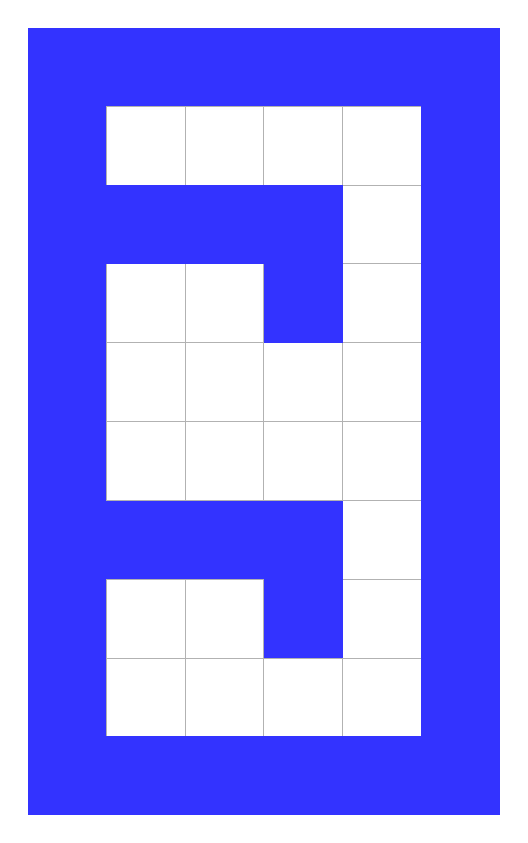
\begin{tikzpicture}
    \draw[draw=black!30] (0, 0) -- (4, 0);
    \draw[draw=black!30] (0, -1) -- (4, -1);
    \draw[draw=black!30] (0, -2) -- (4, -2);
    \draw[draw=black!30] (0, -3) -- (4, -3);
    \draw[draw=black!30] (0, -4) -- (4, -4);
    \draw[draw=black!30] (0, 0) -- (0, -4);
    \draw[draw=black!30] (1, 0) -- (1, -4);
    \draw[draw=black!30] (2, 0) -- (2, -4);
    \draw[draw=black!30] (3, 0) -- (3, -4);
    \draw[draw=black!30] (4, 0) -- (4, -4);

    % exemple de murs
    \draw[fill=blue!80, draw=none] (0, -1) rectangle (1, -2);
    \draw[fill=blue!80, draw=none] (1, -1) rectangle (2, -2);
    \draw[fill=blue!80, draw=none] (2, -1) rectangle (3, -2);
    \draw[fill=blue!80, draw=none] (2, -2) rectangle (3, -3);

\begin{scope}[yshift = -114]
    \draw[draw=black!30] (0, 0) -- (4, 0);
    \draw[draw=black!30] (0, -1) -- (4, -1);
    \draw[draw=black!30] (0, -2) -- (4, -2);
    \draw[draw=black!30] (0, -3) -- (4, -3);
    \draw[draw=black!30] (0, -4) -- (4, -4);
    \draw[draw=black!30] (0, 0) -- (0, -4);
    \draw[draw=black!30] (1, 0) -- (1, -4);
    \draw[draw=black!30] (2, 0) -- (2, -4);
    \draw[draw=black!30] (3, 0) -- (3, -4);
    \draw[draw=black!30] (4, 0) -- (4, -4);

    % exemple de murs
    \draw[fill=blue!80, draw=none] (0, -1) rectangle (1, -2);
    \draw[fill=blue!80, draw=none] (1, -1) rectangle (2, -2);
    \draw[fill=blue!80, draw=none] (2, -1) rectangle (3, -2);
    \draw[fill=blue!80, draw=none] (2, -2) rectangle (3, -3);
  \end{scope}

    % contours
    \draw[fill=blue!80, draw=none] (-1, 1) rectangle (5, 0);
    \draw[fill=blue!80, draw=none] (4, 1) rectangle (5, -9);
    \draw[fill=blue!80, draw=none] (-1, -8) rectangle (5, -9);
    \draw[fill=blue!80, draw=none] (-1, 1) rectangle (0, -9);

  \end{tikzpicture}}
  \caption{Concaténation "sans ligne blanche"}\label{fig:concat}
\end{figure}

\begin{figure}[htbp]
  \begin{verbatim}


         0000
         1110
         0010
         0000

         0000
         1110
         0010
         0000
  \end{verbatim}
  \vspace*{-5cm}
  \hspace{3cm}
  \centering
  \scalebox{0.8}{%
  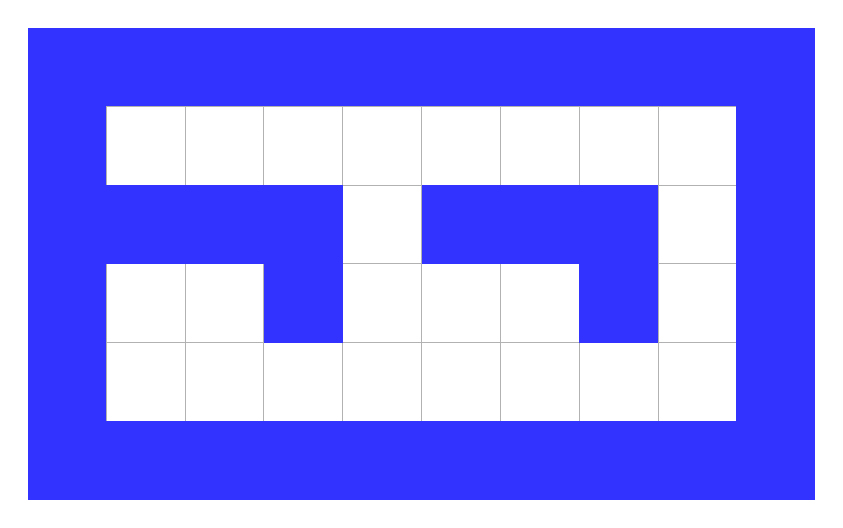
\begin{tikzpicture}
    \draw[draw=black!30] (0, 0) -- (4, 0);
    \draw[draw=black!30] (0, -1) -- (4, -1);
    \draw[draw=black!30] (0, -2) -- (4, -2);
    \draw[draw=black!30] (0, -3) -- (4, -3);
    \draw[draw=black!30] (0, -4) -- (4, -4);
    \draw[draw=black!30] (0, 0) -- (0, -4);
    \draw[draw=black!30] (1, 0) -- (1, -4);
    \draw[draw=black!30] (2, 0) -- (2, -4);
    \draw[draw=black!30] (3, 0) -- (3, -4);
    \draw[draw=black!30] (4, 0) -- (4, -4);

    % exemple de murs
    \draw[fill=blue!80, draw=none] (0, -1) rectangle (1, -2);
    \draw[fill=blue!80, draw=none] (1, -1) rectangle (2, -2);
    \draw[fill=blue!80, draw=none] (2, -1) rectangle (3, -2);
    \draw[fill=blue!80, draw=none] (2, -2) rectangle (3, -3);

\begin{scope}[xshift = 114]
    \draw[draw=black!30] (0, 0) -- (4, 0);
    \draw[draw=black!30] (0, -1) -- (4, -1);
    \draw[draw=black!30] (0, -2) -- (4, -2);
    \draw[draw=black!30] (0, -3) -- (4, -3);
    \draw[draw=black!30] (0, -4) -- (4, -4);
    \draw[draw=black!30] (0, 0) -- (0, -4);
    \draw[draw=black!30] (1, 0) -- (1, -4);
    \draw[draw=black!30] (2, 0) -- (2, -4);
    \draw[draw=black!30] (3, 0) -- (3, -4);
    \draw[draw=black!30] (4, 0) -- (4, -4);

    % exemple de murs
    \draw[fill=blue!80, draw=none] (0, -1) rectangle (1, -2);
    \draw[fill=blue!80, draw=none] (1, -1) rectangle (2, -2);
    \draw[fill=blue!80, draw=none] (2, -1) rectangle (3, -2);
    \draw[fill=blue!80, draw=none] (2, -2) rectangle (3, -3);
  \end{scope}

    % contours
    \draw[fill=blue!80, draw=none] (-1, 1) rectangle (9, 0);
    \draw[fill=blue!80, draw=none] (8, 1) rectangle (9, -5);
    \draw[fill=blue!80, draw=none] (-1, -4) rectangle (9, -5);
    \draw[fill=blue!80, draw=none] (-1, 1) rectangle (0, -5);

  \end{tikzpicture}}
  \caption{Concaténation "avec ligne blanche"}\label{fig:concat2}
\end{figure}

%% Le langage de commandes du système d'exploitation offre une commande permettant de concaténer simplement deux fichiers (ou plus) ; il s'agit de la commande \verb|cat|. La connaissance de ce langage de commandes va donc nous faciliter la vie, lorsqu'on construit des programmes !


\end{document}
